\documentclass[table,aspectratio=169]{beamer}
%% Choose aspect ratio:
% [aspectratio=43]  % 4:3 (default)
% [aspectratio=169] % 16:9, wide

\usetheme[minimal, nofont, noheadline]{tugraz2018}
%\usetheme[iaik,]{tugraz2018}
%% Choose main theme variant:
% [standard]        % standard (default)
% [iaik]       % with institute's graphical acronym on the left
% [minimal]         % with reduced visuals

%% Choose your font style:
%                   % Helvetica (default for Corporate Design)
% [webfont]         % Source Sans Pro (as used on tugraz.at)
% [nofont]          % no font loaded - Computer Modern Sans

%% Choose your department's color instead of TU Graz red (optional):
% [arch]            % 
% [bau]             %
% [etit]            %
% [mbww]            %
% [tcvp]            %
% [mpug]            %
% [infbio]          %


\usepackage[utf8]{inputenc}
\usepackage[english]{babel}
%% Choose your language:
% [ngerman]   % German
% [english]   % English


%% Add your own packages, macros, etc.
\usepackage{xcolor,colortbl}
\usepackage{mathtools}
\usepackage{booktabs,nicematrix}
\usepackage{rotating}
\usepackage[style=alphabetic,backend=biber]{biblatex} % Bibliography
\addbibresource{\jobname.bib}                         % Bibliography
\usepackage{fontawesome}
\usepackage{filecontents}
\usepackage{setspace}
\usepackage{subcaption}
\usepackage{multirow}
\usepackage{bm}
\usepackage{pgfplots}
\usepackage[linesnumbered,ruled,vlined]{algorithm2e}
\usepackage{framed, color}


\tikzset{
  invisible/.style={opacity=0},
  visible on/.style={alt={#1{}{invisible}}},
  alt/.code args={<#1>#2#3}{%
    \alt<#1>{\pgfkeysalso{#2}}{\pgfkeysalso{#3}} % \pgfkeysalso doesn't change the path
  },
}

\usetikzlibrary{calc,patterns,arrows.meta, shapes.geometric}
\usetikzlibrary{positioning}
\usetikzlibrary{cipher}
\setbeamersize
{
	text margin left=0.4cm,
	text margin right=0.4cm
}

%% Enter presentation metadata
\title{Automated Search for Full Impossible Differential, Zero-Correlation, and Integral Attacks}
\author{\underline{\textbf{Hosein Hadipour}}, Sadegh Sadeghi, and Maria Eichlseder}
\date{ISC-Webinar 2022 - Virtual}
%\institute{IAIK}
\instituteurl{hsn.hadipour@gmail.com}

%% Logos
%\institutelogo{beamerthemetugraz/institute/IAIK}  % graphical acronym for [] theme (left margin)
% \additionallogo{figures/logo}  % additional institute/department logo (footline; optional)
% \logobar{Supported by: ...}  % sponsors (titlepage; optional)

%% Macros
\definecolor{gold}{HTML}{F0AB00}
\definecolor{bound}{HTML}{78b473}
\definecolor{best}{HTML}{e59352}
\definecolor{lin}{HTML}{285f82}
\definecolor{sub}{HTML}{78b473}
\definecolor{lightred}{rgb}{0.9, 0.2, 0.2}
\definecolor{lightblue}{rgb}{0, 0.5, 0.9}
%%%commands to represent CSP/COP variables/constraints%%%
\newcommand{\ax}{\texttt{AX}\xspace} %AX
\newcommand{\ay}{\texttt{AY}\xspace} %AY
\newcommand{\az}{\texttt{AZ}\xspace} %AZ
\newcommand{\aw}{\texttt{AW}\xspace} %AW
\newcommand{\dx}{\texttt{DX}\xspace} %DX
\newcommand{\lx}{\texttt{LX}\xspace} %LX
\newcommand{\dy}{\texttt{DY}\xspace} %DY
\newcommand{\ly}{\texttt{LY}\xspace} %LY
\newcommand{\dz}{\texttt{DZ}\xspace} %DZ
\newcommand{\lz}{\texttt{LZ}\xspace} %LZ
\newcommand{\dw}{\texttt{DW}\xspace} %DW
\newcommand{\lw}{\texttt{LW}\xspace} %LW
\newcommand{\kx}{\texttt{KX}\xspace} %KX
\newcommand{\ky}{\texttt{KY}\xspace} %KY
\newcommand{\dtk}{\texttt{DTK}\xspace} %DTK
\newcommand{\dstk}{\texttt{DSTK}\xspace} %DSTK

\newcommand{\axu}{\texttt{AXU}\xspace} %AXU
\newcommand{\ayu}{\texttt{AYU}\xspace} %AYU
\newcommand{\azu}{\texttt{AZU}\xspace} %AZU
\newcommand{\dxu}{\texttt{DXU}\xspace} %DXU
\newcommand{\dyu}{\texttt{DYU}\xspace} %DYU
\newcommand{\dzu}{\texttt{DZU}\xspace} %DZU
\newcommand{\lxu}{\texttt{LXU}\xspace} %LXU
\newcommand{\axl}{\texttt{AXL}\xspace} %AXL
\newcommand{\ayl}{\texttt{AYL}\xspace} %AYL
\newcommand{\azl}{\texttt{AZL}\xspace} %AZL
\newcommand{\dxl}{\texttt{DXL}\xspace} %DXL
\newcommand{\dyl}{\texttt{DYL}\xspace} %DYL
\newcommand{\dzl}{\texttt{DZL}\xspace} %DZL
\newcommand{\lxl}{\texttt{LXL}\xspace} %LXL
\newcommand{\astk}{\texttt{ASTK}\xspace} %ASTK

\newcommand{\axb}{\texttt{AXB}\xspace} %AXB
\newcommand{\azb}{\texttt{AZB}\xspace} %AZB
\newcommand{\kxb}{\texttt{KXB}\xspace} %KXB
\newcommand{\kyb}{\texttt{KYB}\xspace} %KYB
\newcommand{\kdxb}{\texttt{KDXB}\xspace} %KDXB
\newcommand{\kdzb}{\texttt{KDZB}\xspace} %KDZB
\newcommand{\cb}{\texttt{CB}\xspace} %CB
\newcommand{\ikb}{\texttt{IKB}\xspace} %IKB

\newcommand{\axf}{\texttt{AXF}\xspace} %AXF
\newcommand{\azf}{\texttt{AZF}\xspace} %AZB
\newcommand{\kxf}{\texttt{KXF}\xspace} %KXF
\newcommand{\kyf}{\texttt{KYF}\xspace} %KYF
\newcommand{\kdxf}{\texttt{KDXF}\xspace} %KDXF
\newcommand{\kdzf}{\texttt{KDZF}\xspace} %KDZF
\newcommand{\cf}{\texttt{CF}\xspace} %CF
\newcommand{\ikf}{\texttt{IKF}\xspace} %IKF

\newcommand{\ik}{\texttt{IK}\xspace} %IK
\newcommand{\ke}{\texttt{KE}\xspace} %KE
\newcommand{\ks}{\texttt{KS}\xspace} %KS

\newcommand{\D}{\texttt{D}\xspace} %Data complexity D[0], D[1]
\newcommand{\T}{\texttt{T}\xspace} %Time complexity T[0], T[1], T[2], T[3]
\newcommand{\W}{\texttt{W}\xspace} %hamming weight of IO differences
\newcommand{\gp}{\texttt{g}\xspace} %g parameter
\newcommand{\C}{\texttt{C}\xspace} %c parameters c\In, c\Out
\newcommand{\s}{\texttt{c}\xspace} %s: cell size in our CP formulas
\newcommand{\z}{\texttt{z}\xspace} %z: number of tweakey paths in SKINNY
\newcommand{\blocksize}{\texttt{n}\xspace} %block size in our CP models
\newcommand{\ksize}{\texttt{k}\xspace} %key size in our CP models

\newcommand{\cp}[1]{\textit{\texttt{#1}}\xspace} % CP x
\newcommand{\csp}{\textit{\texttt{CSP}}\xspace} % CSP problem
\newcommand{\cop}{\textit{\texttt{COP}}\xspace} % COP problem
\newcommand{\cpmodel}{\mathcal{M}\xspace} % CP model M
\newcommand{\cpvars}{\mathcal{M}.\texttt{var}\xspace} % CP variables
\newcommand{\cpcons}{\mathcal{M}.\texttt{con}\xspace} % CP constraints
\newcommand{\cpobj}{\mathcal{M}.\texttt{obj}\xspace} % CP objective
\newcommand{\booltoint}{\textit{\texttt{bool2int}}\xspace} % CP bool2int operator
\newcommand{\cpif}{\textit{\texttt{if}}\xspace} % CP If
\newcommand{\cpthen}{\textit{\texttt{then}}\xspace} % CP Then
\newcommand{\cpelse}{\textit{\texttt{else}}\xspace} % CP Else
\newcommand{\cpelseif}{\textit{\texttt{elseif}}\xspace} % CP Elseif
\newcommand{\cpendif}{\textit{\texttt{endif}}\xspace} % CP Endif

\newcommand{\cplink}{\textit{\texttt{Link}}\xspace} % CP Link
\newcommand{\cpxor}{\textit{\texttt{XOR}}\xspace} % CP XOR
\newcommand{\cpsbox}{\textit{\texttt{S-box}}\xspace} % CP S-box
\newcommand{\cpmds}{\textit{\texttt{MDS}}\xspace} % CP MDS
\newcommand{\cpbranch}{\textit{\texttt{Branch}}\xspace} % CP Branching
\newcommand{\cptrue}{\textit{\texttt{True}}\xspace} % CP True
\newcommand{\cpfalse}{\textit{\texttt{False}}\xspace} % CP False
\newcommand{\cplog}{\textit{\texttt{LG}}\xspace} % CP Log(g) - 0.53
\newcommand{\cpmax}{\textit{\texttt{max}}\xspace} % CP Max
\newcommand{\cpmin}{\textit{\texttt{min}}\xspace} % CP Min
\newcommand{\cpmdiff}{\textit{\texttt{Mdiff}}\xspace} % CP Mdiff
\newcommand{\cpminvdiff}{\textit{\texttt{Minvdiff}}\xspace} % CP Minvdiff
\newcommand{\cpmlin}{\textit{\texttt{Mlin}}\xspace} % CP Mlin
\newcommand{\cpminvlin}{\textit{\texttt{Minvlin}}\xspace} % CP Minvlin
\newcommand{\cpmdata}{\textit{\texttt{Mdata}}\xspace} % CP Mdata
\newcommand{\cpminvdata}{\textit{\texttt{Minvdata}}\xspace} % CP Minvdata

% notation for ID and figures
\newcommand{\In}{_{\textsc{b}}} % input difference of Ei (initial key-recovery rounds)
\newcommand{\Out}{_{\textsc{f}}} % output difference of Eo (final key-recovery rounds)
\newcommand{\Up}{_{\textsc{u}}} % input difference of Eu (initial distinguisher rounds)
\newcommand{\Low}{_{\textsc{l}}} % output difference of El (final distinguisher rounds)
\newcommand{\Dist}{_{\textsc{d}}} % distinguisher rounds Eu, El (middle)
\newcommand{\KB}{_{\textsc{KB}}} % Key-Bridging
\newcommand{\GD}{_{\textsc{GD}}} % Guess-and-Determine
\newcommand{\DP}{_{\textsc{DP}}} % Difference Propagation
\newcommand{\Off}{_{\text{off}}} % offset for round counter in Eu, El, and Ef
\newcommand{\Tot}{_\textit{Tot}}
\newcommand{\STK}{\textit{STK}}
\newcommand{\ETK}{\textit{ETK}}
\newcommand{\TK}{\textit{TK}}
\newcommand{\lane}{\textit{Lane}}
\newcommand{\cs}{c} % indicates the cell size in the main body
\newcommand{\as}{m} % indicates the state array size in the main body

\newcommand{\sparen}{\vspace*{-.3cm}}
\newcommand{\cipher}[1]{\textsc{#1}}

\begin{document}

\begin{frame}[plain]
  \maketitle
\end{frame}


\section*{}
\begin{frame}{Outline}
  \tableofcontents
\end{frame}

\section{Introduction}
\sectionheader[\huge\color{tug}\faBook]{Introduction}

\begin{frame}{Cryptographic Primitives}
\begin{itemize}
\onslide<1->{\item Symmetric-Key Primitives}
\begin{itemize}
\footnotesize
\onslide<2->{\item Block ciphers (AES \cite{daemen1999aes}, CLEFIA \cite{conf_fse_ShiraiSAMI07}, SKINNY \cite{skinny})}
\onslide<2->{\item Stream ciphers (Trivium\cite{canniere2008trivium}, ZUC \cite{zuc128_specification}, Enocoro-128v2 \cite{watanabe2010hardware})}
\onslide<2->{\item Unkeyed primitives (Ascon \cite{ascon_caesar_submission_2016}, Keccak \cite{eurocrypt_BertoniDPA13})}
\end{itemize}
\onslide<1->{\item Public-Key Primitives}
\begin{itemize}
\footnotesize
\onslide<3->{\item Public-key encryption algorithms (RSA, ECC)}
\onslide<3->{\item Digital signature algorithms (RSA, ECC)}
\onslide<3->{\item Key-exchange protocols (DH)}
\end{itemize}
\end{itemize}
\end{frame}

\begin{frame}{\cipher{SKINNY} Family of Twekable Block Ciphers \cite{skinny}}
\begin{figure}
\centering
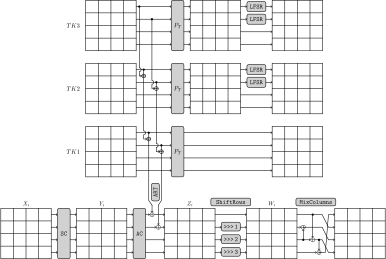
\includegraphics[width=0.6\textwidth]{./figures/skinny_round_function_complete.pdf}
\end{figure}
\end{frame}

\begin{frame}{\cipher{CRAFT} Tweakable Block Cipher\cite{tosc_BeierleLMR19}}
\centering
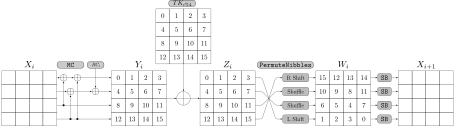
\includegraphics[width=0.9\textwidth]{./figures/craft_round_function.pdf}
\begin{itemize}
  \item Tweakey schedule:
  \[TK_{0} = K_{0} \oplus T, ~ TK_{1} = K_{1} \oplus T,~ TK_{2} = K_{0} \oplus Q(T), ~ TK_{3} = K_{1} \oplus Q(T)\]
  \item $Q$: a permutation on the position of nibbles
  \item Round tweakey: $TK_{i\% 4}$
\end{itemize}
\end{frame}

\begin{frame}{Symmetric-Key V.S. Public-Key Cryptography}
\begin{itemize}
  \item Symmetric-key primitives are faster, but require a pre-shared key
  \item Public-key primitives are slower, but require no pre-shared key
  \item Modern cryptographic systems employ both types of primitives
  \item Public-key cryptography is used to securely establish a common key
  \item Symmetric-key cryptography secures the transactions with a common key
\end{itemize}
\begin{figure}
\centering
\includegraphics[width=0.35\textwidth]{./figures/tls.png}
\end{figure}
\end{frame}

\begin{frame}{Cryptanalysis}
\begin{itemize}
\item Complexity-theoretic approach (Public-Key primitives)
\item Cryptanalytic approach (Symmetric-Key primitives)
\only<2>{
\begin{itemize}
  \item Linear attack on DES \cite{conf_eurocrypt_Matsui93}
  \item Differential analysis of AES-256 in the related-key setting \cite{conf_crypto_BiryukovKN09}
  \item Integral analysis based on division property on full MISTY \cite{conf_crypto_Todo15}
  \item Cube attack against reduced round of SHA-3 \cite{conf_eurocrypt_HuangWXWZ17}
\end{itemize}
}
\end{itemize}
\end{frame}

\begin{frame}{Automated Methods in Cryptanalysis}
Mounting cryptanalytic attacks against symmetric-key primitives:
\begin{itemize}
\item requires tracing the propagation of a certain property at the bit-level
\item implies solving a hard combinatorial optimization problem
\item is very time-consuming
\item is potentially an error-prone process
\end{itemize}
\pause
\vspace{-0.4cm}
\begin{block}{Automated Methods in Cryptanalysis}
Getting the help or using of machines to \textcolor{tugred}{find}, \textcolor{tugblue}{build} or \textcolor{tuggreen}{optimize} the attacks
\end{block}
\end{frame}

\begin{frame}{Different Approaches for Automatic Cryptanalysis}
\begin{itemize}
\item Dedicated algorithms
\item {\color<2>{tugred} Constraint Satisfaction/Optimization Problem (CSP/COP)}
\begin{itemize}
\item {\color<2>{tugred} CP}
\begin{itemize}
\item {\color<2>{tugred} MILP}
\item {\color<2>{tugred} SAT}
\item {\color<2>{tugred} SMT}
\end{itemize}
\end{itemize}
\item Artificial Intelligence (AI)
\end{itemize}
\end{frame}
  
\section{Constraint Programming (CP)}
\sectionheader[\huge\color{tug}\faLaptop]{Constraint Programming (CP)}

\begin{frame}{Constraint Programming (CP)}
\begin{itemize}
% \item Programming in CP refers to the arrangement of a plan
% \item For example the \href{https://developers.google.com/optimization/scheduling/employee_scheduling}{employee scheduling problem}
\item In \textbf{CP} we specify the properties of the solution to be found:
\begin{itemize}
\item<1-> We define a set of variables: $\mathcal{X} = \{\mathcal{X}_{1}, \ldots, \mathcal{X}_{n}\}$
\item<2-> We specify the domain of each variable: $\mathbb{F}_{2}, \mathbb{Z}, \mathbb{R}, \ldots$
\item<3-> We define a set of constraints: $\mathcal{C} = \{\mathcal{C}_{1}, \ldots, \mathcal{C}_{2}\}$
\item<4-> We define an objective function (if it is required)
\end{itemize}
\item<5-> \textcolor{tugred}{MILP} and \textcolor{tugblue}{SAT} are special cases of CP
\end{itemize}
\end{frame}

\begin{frame}[fragile]
\frametitle{Constraint Satisfaction/Optimization Problem (CSP/COP)- Example}
\begin{columns}
\column[c]{0.45\textwidth}
\begin{center}
\only<1>{\includegraphics[width=0.9\textwidth]{./figures/austria.pdf}}
\only<2>{\includegraphics[width=0.9\textwidth]{./figures/austria_legend.pdf}}
\only<3>{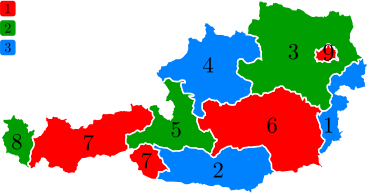
\includegraphics[width=0.9\textwidth]{./figures/austria3colored.pdf}}
\end{center}
\column[c]{0.55\textwidth}
\pause
{\scriptsize
\begin{verbatim}
int: nc = 3;
array[1..9] of var 1..nc: r;
constraint r[1] != r[3]; constraint r[1] != r[6];
constraint r[2] != r[5]; constraint r[2] != r[6]; 
constraint r[2] != r[7]; constraint r[3] != r[9]; 
constraint r[3] != r[6]; constraint r[3] != r[4];
constraint r[4] != r[6]; constraint r[4] != r[5];
constraint r[5] != r[6]; constraint r[5] != r[7];
constraint r[7] != r[8];
solve satisfy;
\end{verbatim}}
\pause
\vspace{-0.4cm}
{\scriptsize
\begin{verbatim}
r = [3, 3, 2, 3, 2, 1, 1, 2, 1];
\end{verbatim}}
\end{columns}
\end{frame}

\begin{frame}{\small Truncated Differential Trail for AES with Minimum Number of Active S-boxes}
\vspace{-0.2cm}
\begin{figure}
\centering

\includegraphics[width=0.8\textwidth]{./figures/aes2rtruncdiff.pdf}
\end{figure}
\onslide<2>{%}
\textcolor{tugred}{Variables}:
\begin{itemize}
\footnotesize
  \item $s_{r, i, j} \in \{0, 1\}$ is S-box in row $i$, column $j$, round $r$ active?
  \item $m_{r, j}\in \{0, 1\}$ is Mix-columns $j$ in round $r$ active?
\end{itemize}
\textcolor{tugblue}{Objective function and constraints}:
\begin{itemize}
\footnotesize
  \item $\min \sum_{r, i, j} s_{r, i, j}$
  \item $5 \cdot M_{r, j} \leq \sum_{i} s_{r, i, (i + j)\%4} + \sum_{i}s_{r + 1, i, j} \leq 8 \cdot M_{r, j}; \quad \sum_{i, j} s_{0, i, j} \geq 1$
\end{itemize}
}
\end{frame}

\section{Impossible Differential Attack (ID)}
\sectionheader[\huge\color{tug}\faMagic]{Impossible Differential Attack (ID)}

\begin{frame}{Impossible Differential (ID) Attack}
\begin{itemize}
  \item \textcolor{tugred}{Core idea}: Exploit an \underline{impossible event} in block cipher to retrieve the secret key
\end{itemize}
\only<2->{%
\begin{columns}[onlytextwidth]
\column[c]{0.55\textwidth}
\begin{itemize}
\item Find an impossible differential \textcolor{tugred}{$\Delta\Up \not\to \Delta\Low$}
\item Use it as a \textbf{distinguisher} to retrieve the key
\begin{itemize}
  \item Keys that suggest $(\Delta\Up, \Delta\Low)$ are wrong
  \item Discard as many wrong keys as possible
\end{itemize}
\item Brute force the remaining key candidates
\end{itemize}
\column[c]{0.45\textwidth}
\centering
\begin{tikzpicture}[xscale=1.2, yscale=1.1]  
  \draw (0,1.5)    coordinate (M)
        (0,.75)   coordinate (X)
        (0,-.75)  coordinate (Y)
        (0,-1.5)   coordinate (C)
        (-1.4,0) coordinate (w)
        (1.4,0)  coordinate (e)
    (w)+(.2,0)   coordinate (a); % round arrows  
  \draw[rounded corners=2pt] (w|-M) rectangle (e|-C);
  \draw[dashed] (w|-X) -- (e|-X)
                (w|-Y) -- (e|-Y);
  \draw (M) node[above] {$\Delta\In$}
        (X) node[below] {$\Delta\Up$}
        (Y) node[above] {$\Delta\Low$}
        (C) node[below] {$\Delta\Out$};
  \begin{scope}[>=latex, <->, shorten <=2pt, shorten >=2pt, gray, font=\footnotesize]
    \draw (a|-M) -- node[right] {$r\In$ rounds} (a|-X);
    \draw (a|-X) -- node[right] {$r\Dist$ rounds} (a|-Y);
    \draw (a|-Y) -- node[right] {$r\Out$ rounds}  (a|-C);
  \end{scope}
  \draw[font=\footnotesize] (e|-X) node[above left] {\textcolor{tugred}{$k\In$},  \textcolor{tugblue}{$c\In$}}
                            (e|-Y) node[below left] {\textcolor{tugred}{$k\Out$}, \textcolor{tugblue}{$c\Out$}};
  \begin{scope}[decoration={brace, amplitude=4pt, raise=2pt}]
    \draw[decorate] (e|-X) -- node[right=8pt] {\textcolor{tugred}{$\Delta\Up \not\to \Delta\Low$}} (e|-Y);
    \draw[decorate] (e|-M) -- node[right=8pt] {$\Delta\In \leftarrow \Delta\Up$} (e|-X);
    \draw[decorate] (e|-Y) -- node[right=8pt] {$\Delta\Low \rightarrow \Delta\Out$} (e|-C);
  \end{scope}
\end{tikzpicture}
\end{columns}}
\end{frame}

\begin{frame}{Core Idea of ID Attack}
\vspace{-0.2cm}
\begin{center}
\scalebox{0.8}{
  \begin{tabular}{|c|c|c|c|c|c|c|c|c|c|c|c|c|c|c|c|c|}
    \hline
    $X$   & $\mathtt 0$ & $\mathtt 1$ & $\mathtt 2$ & $\mathtt 3$ & $ \mathtt 4$ & $\mathtt 5$ & $\mathtt 6$ & $\mathtt 7$ & $ \mathtt 8$ & $\mathtt 9$ & $\mathtt a$ & $\mathtt b$ & $\mathtt c$ & $\mathtt d$ & $\mathtt e$ & $\mathtt f$ \\
    \hline
    $\mathcal S(X)$ & $\mathtt c$ & $\mathtt 5$ & $\mathtt 6$ & $\mathtt b$ & $\mathtt 9$ & $\mathtt 0$ & $\mathtt a$ & $\mathtt d$ & $\mathtt 3$ & $\mathtt e$ & $\mathtt f$ & $\mathtt 8$ & $\mathtt 4$ & $\mathtt 7$ & $\mathtt 1$ & $\mathtt 2$\\
    \hline
  \end{tabular}
}
\[C = S(S(X \oplus K_{1}) \oplus K_{2}) \oplus \textcolor{tugred}{K_{1}}\]
\end{center}

\begin{center}
\only<1-3>{
\begin{tikzpicture}[very thick, >=latex, xscale=1, yscale=1]
  \pgfmathsetmacro{\esep}{0.7}
  \node (x) at (0,0) {$X$};  
  \node[xor, right=\esep of x] (wk) {};
  \node[above=\esep of wk] (k0) {\textcolor{tugred}{$K_{1}$}};
  \node[box, right=\esep of wk] (sbox) {$S$};
  \node[xor, right=\esep of sbox] (xor) {};
  \node[above=\esep of xor] (k) {\textcolor{tugred}{$K_{2}$}};
  \node[right=\esep of xor] (c) {};
  \draw[->] (x) -- (sbox);
  \draw[->] (sbox) -- (xor);
  \draw[->] (xor) -- (c);
  \draw[->] (k0) -- (wk);
  \draw[->] (k) -- (xor);
  \node (x) at (c) {$Y$};
  \node[box, right=\esep of x] (sbox) {$S$};
  \node[xor, right=\esep of sbox] (xor) {};
  \node[above=\esep of xor] (k) {\textcolor{tugred}{$K_{1}$}};
  \node[right=\esep of xor] (c) {$C$};
  \draw[->] (x) -- (sbox);
  \draw[->] (sbox) --node[anchor=north] {} (xor);
  \draw[->] (xor) -- (c);
  \draw[->] (k) -- (xor);
\end{tikzpicture}
}
\end{center}

\vspace{-0.2cm}
\begin{itemize}
  \item<2-> \textcolor{tugblue}{Impossible differential}: if $\Delta X = \texttt{f}$ then $\Delta Y \notin I = \{\texttt{0}, \texttt{2}, \texttt{3}, \texttt{5}, \texttt{6}, \texttt{7}, \texttt{8}, \texttt{9}, \texttt{a}, \texttt{b}, \texttt{c}, \texttt{d}\}$
  \vspace{-0.2cm}
  \item<3> \textcolor{tugblue}{Filter wrong keys}: $S^{-1}(C \oplus K_{1}) \oplus S^{-1}(C' \oplus K_{1}) \notin I$ where $P \oplus P' = \texttt{f}$
\end{itemize}
\end{frame}

\begin{frame}{Notations}
\begin{columns}[onlytextwidth]
\column[c]{0.55\textwidth}
\begin{itemize}
\item $\Pr(\Delta\Up \rightarrow \Delta\In) = 1, ~ \Pr(\Delta\Up \leftarrow \Delta\In) = 2^{-c\In}$
\item $\Pr(\Delta\Low \rightarrow \Delta\Out) = 1, ~ \Pr(\Delta\Low \leftarrow \Delta\Out) = 2^{-c\Out}$
\item $k\In$ is involved to check $\Delta\In \rightarrow \Delta\Up$
\item $k\Out$ is involved to check $\Delta\Out \rightarrow \Delta\Low$
\end{itemize}
\column[c]{0.45\textwidth}
\centering
\begin{tikzpicture}[xscale=1.2, yscale=1.1]  
  \draw (0,1.5)    coordinate (M)
        (0,.75)   coordinate (X)
        (0,-.75)  coordinate (Y)
        (0,-1.5)   coordinate (C)
        (-1.4,0) coordinate (w)
        (1.4,0)  coordinate (e)
    (w)+(.2,0)   coordinate (a); % round arrows  
  \draw[rounded corners=2pt] (w|-M) rectangle (e|-C);
  \draw[dashed] (w|-X) -- (e|-X)
                (w|-Y) -- (e|-Y);
  \draw (M) node[above] {$\Delta\In$}
        (X) node[below] {$\Delta\Up$}
        (Y) node[above] {$\Delta\Low$}
        (C) node[below] {$\Delta\Out$};
  \begin{scope}[>=latex, <->, shorten <=2pt, shorten >=2pt, gray, font=\footnotesize]
    \draw (a|-M) -- node[right] {$r\In$ rounds} (a|-X);
    \draw (a|-X) -- node[right] {$r\Dist$ rounds} (a|-Y);
    \draw (a|-Y) -- node[right] {$r\Out$ rounds}  (a|-C);
  \end{scope}
  \draw[font=\footnotesize] (e|-X) node[above left] {\textcolor{tugred}{$k\In$},  \textcolor{tugblue}{$c\In$}}
                            (e|-Y) node[below left] {\textcolor{tugred}{$k\Out$}, \textcolor{tugblue}{$c\Out$}};
  \begin{scope}[decoration={brace, amplitude=4pt, raise=2pt}]
    \draw[decorate] (e|-X) -- node[right=8pt] {\textcolor{tugred}{$\Delta\Up \not\to \Delta\Low$}} (e|-Y);
    \draw[decorate] (e|-M) -- node[right=8pt] {$\Delta\In \leftarrow \Delta\Up$} (e|-X);
    \draw[decorate] (e|-Y) -- node[right=8pt] {$\Delta\Low \rightarrow \Delta\Out$} (e|-C);
  \end{scope}
\end{tikzpicture}
\end{columns}
\end{frame}

\begin{frame}{Key Recovery of ID Attack}
  \begin{itemize}
  \item \textit{Pair Generation.} \onslide<2->{Generate $N$ pairs satisfying the input/output activeness pattern}
  \item \textit{Guess-and-Filter.} \onslide<3->{For each pair:
  \begin{itemize}
    \item Guess the involved keys and partially encrypt (decrypt)
    \item Discard the key if it yields the impossible differential
  \end{itemize}}
  \item \textit{Exhaustive Search.} \onslide<4>{Brute force the remaining key candidates}
\end{itemize}
\end{frame}

\begin{frame}{Pair Generation}
\begin{itemize}
\item[\faCheck] Generate $N$ pairs satisfying the input/output activeness pattern
\item We construct the pairs by using the plaintext (ciphertext) structures
\begin{columns}[onlytextwidth]
\column[c]{0.5\textwidth}
\begin{itemize}
  \item For more than one structures
  \[N 2^{n + 1 - |\Delta\In| - |\Delta\Out|}\]
  \item For one structure 
  \[\min_{\Delta \in \{\Delta\In, \Delta\Out\}} \left\{ \sqrt{N 2^{n + 1 - |\Delta|}} \right\}\]
\end{itemize}
\column[c]{0.5\textwidth}
\centering
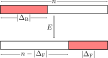
\includegraphics[width=0.8\textwidth]{./figures/limited_birthday_problem.pdf}
\end{columns}
\end{itemize}
\end{frame}

\begin{frame}{Complexity Analysis of ID Attack}
\vspace{-0.5cm}
\begin{itemize}
\item[\faCheckCircleO]<1-> Generate $N$ pairs 
\[T_{0} = \max\left\{\min_{\Delta \in \{\Delta\In, \Delta\Out\}} \left\{ \sqrt{N 2^{n + 1 - |\Delta|}} \right\}, N 2^{n + 1 - |\Delta\In| - |\Delta\Out|} \right\}\]
\item[\faCheckCircleO]<2-> Guess and filter
\[T_1 + T_2 = N + 2^{|k\In \cup k\Out|} \frac{N}{2^{c\In + c\Out}}\]
\item[\faCheckCircleO]<3-> Brute force
\[T_3 = 2^{k - |k\In \cup k\Out|} \cdot P \cdot 2^{|k\In\cup k\Out|} = 2^{k}\cdot P, ~ P = \left(1 - 2^{-(c\In + c\Out)}\right)^{N}, \textcolor{tugred}{P < 2^{-1}}\]
\onslide<4>{%}
\[T_{tot} = \left(T_{0} + \left(T_{1} + T_{2}\right) C_{E'} + T_{3}\right) C_{E}\]
}
\end{itemize}
\end{frame}

\begin{frame}{Reformulating the Complexity of ID Attack}
\begin{itemize}
  \item[\faCheck]<1-> Let $P = 2^{-g},~ 1 < g \leq |k\In \cup k\Out|$
  \item[\faCheck]<2-> $P = \left(1 - 2^{-(c\In + c\Out)}\right)^{N}$, thus $N = 2^{c\In + c\Out + \log_{2}(g) - 0.53}$
  \item[\faCheck]<3-> CP-friendly formulation:
  \begin{align*}
    \begin{split}
      & T_{0} = \max\left\{
      \begin{aligned}
      & \min_{\Delta \in \{\Delta\In, \Delta\Out\}} \{2^{\frac{c\In + c\Out + n + 1 - |\Delta| + \cplog(g)}{2}}\},\\
      & 2^{c\In + c\Out + n + 1 - |\Delta\In| - |\Delta\Out| + \cplog(g)}
      \end{aligned}
      \right\}, ~ T_{0} < 2^{n},\\
      & T_{1} = 2^{c\In + c\Out + \cplog(g)}, ~ T_{2} = 2^{|k\In \cup k\Out| + \cplog(g)},~ T_{3} = 2^{k - g},\\
      & T_\text{tot} = \left(T_{0} + \left(T_{1} + T_{2}\right) C_{E'} + T_{3}\right) C_{E}, ~ T_\text{tot} < 2^{k},\\
      %& M_\text{tot} = \min \big\{2^{c\In + c\Out + \cplog(g)}, 2^{|k\In \cup k\Out|} \big\}, ~ M_\text{tot} < 2^{k}.
    \end{split}
    \end{align*}
\end{itemize}
\end{frame}

% \begin{frame}{Zero-Correlation (ZC) Attack\cite{dcc_BogdanovR14}}
% \begin{itemize}
% \item<1-> Dual of ID attack in the context of linear analysis
% \item<2-> Multiple ZC attacks (FSE~2012) \cite{fse_BogdanovW12}
% \item<3-> Multidimensional ZC attack (ASIACRYPT~2012) \cite{asiacrypt_BogdanovLNW12}
% \item<4-> \textcolor{tugred}{Core idea}: use the difference between two distributions
% \[\left\langle u_{i}, x \right\rangle + \left\langle w_{i}, E\Dist(x) \right\rangle~, i = 0, \ldots, m - 1\]
% \[Z:\mathbb{F}_{2}^{n} \rightarrow \mathbb{F}_{2}^{m}\]
% \[z(x) = (z_{0}, \dots, z_{m - 1}), ~ z_{i} := \langle u_{i}, x \rangle + \langle w_{i}, E\Dist(x)\rangle\]
% \end{itemize}
% \end{frame}

% \begin{frame}{Integral Attack and Its Relation to ZC Attack \cite{Lai1994}, \cite{square_fse_DaemenKR97}}
% \begin{itemize}
%   \item \textcolor{tugred}{Core idea}:
%   Find a set of inputs such that the sum of the resulting outputs is key-independent
%   \only<2>{%}
%   \begin{block}{Link between ZC \& Integral \cite{asiacrypt_BogdanovLNW12}, ~\cite{crypto_SunLRLCWAL15}}
%     Let $F:\mathbb{F}_{2}^{n}\rightarrow \mathbb{F}_{2}^{n}$ be a vectorial Boolean function. 
%   Assume $A$ is a subspace of $\mathbb{F}_{2}^{n}$ and $\beta\in \mathbb{F}_{2}^{n}\setminus \{0\}$
%   such that $(\alpha, \beta)$ is a ZC approximation for any $\alpha \in A$. 
%   Then, for any $\lambda \in \mathbb{F}_{2}^{n}$, $\left\langle \beta, F(x + \lambda)\right\rangle$ is balanced over the set
%   \[A^{\bot} = \{x \in \mathbb{F}_{2}^{n}~|~ \forall ~ \alpha \in A:\left\langle \alpha, x \right\rangle = 0\}.\]
%   \end{block}
%   }
% \end{itemize}
% \end{frame}

\begin{frame}{Previous Methods to Search for ID/ZC, and Integral Distinguishers}
\begin{itemize}
  \item Eprint~2016 (ID) \cite{eprint_Cui}
  \item EUROCRYPT~2017 (ID, ZC) \cite{eurocrypt_SasakiTodo2017}
  \item ToSC~2017 (ID, ZC) \cite{tosc_SunGLYTQH2017}
  \item CRYPTO~2016 ($\mathcal{DC}$-MITM, ID) \cite{crypto_DerbezF16}
  \item ASIACRYPT~2016 (Division Property, Integral) \cite{asiacrypt_XiangZBL16}
  \item ToSC~2020 (ID, ZC) \cite{tosc_SunGWW2020}
\end{itemize}
\end{frame}

\section{Our CP Model to Search For ID Attacks}
\sectionheader[\huge\color{tug}\faGear]{Our CP Model to Search for ID Attacks}

\begin{frame}{Our CP Model for Finding ID Distinguishers (High-level View)}
\begin{columns}[onlytextwidth]
\column[c]{0.5\textwidth}
\begin{itemize}
  \item Divide $E_{\textsc{D}}$ into two parts: $E_{\textsc{D}} = E\Low \circ E\Up$
  \item Model the deterministic truncated trails over $E\Up$ and $E\Low$ forward and backward
  \item \textcolor{tugred}{Include new constraints for the meeting point to guarantee the contradiction}
\end{itemize}
\column[c]{0.5\textwidth}
\begin{center}
\includegraphics[width=0.75\textwidth]{./figures/miss_in_the_middle.pdf}
\end{center}
\end{columns}
\end{frame}

\begin{frame}
\begin{center}
\vspace{2.5cm}
{\huge \faLaptop~Demo~1}
\end{center}
\end{frame}

% \begin{frame}{Constraints for The Meeting Point}
% \begin{columns}[onlytextwidth]
% \column[c]{0.5\textwidth}
% \begin{center}
% \includegraphics[width=0.75\textwidth]{./figures/miss_in_the_middle.pdf}
% \end{center}
% \column[c]{0.5\textwidth}
% \bgroup\small
% \begin{align*}
% \begin{split}
%   &\csp_{M}(\axu_{r\Low}, \dxu_{r\Low}, \axl_{0}, \dxl_{0})\!\coloneqq\!\\ %\begin{cases}
%   &\bigvee_{i = 0}^{\as - 1}\left(
%   \begin{aligned}
%     &(\axu_{r\Up}[i] + \axl_{0}[i] > 0) ~ \wedge \\
%     &(\axu_{r\Up}[i] + \axl_{0}[i] < 3) ~ \wedge \\
%     &~\axu_{r\Up}[i] \neq \axl_{0}[i]
%   \end{aligned}
% \right) \vee \\
%   &\bigvee_{i = 0}^{\as - 1} \left(
%   \begin{aligned}
%     &\axu_{r\Up}[i] = 1 ~ \wedge \\
%     &\axl_{0}[i] ~ = 1 ~ \wedge \\
%     &\dxu_{r\Up}[i] \neq \dxl_{0}[i]
%   \end{aligned}
% \right) = \cptrue
% \end{split}
% \end{align*}
% \egroup
% \end{columns}
% \end{frame}

\begin{frame}{High-level View of Our Unified Model for Key Recovery Attacks}
\begin{itemize}
  \item Model the distinguisher
  \item Model the difference propagation through the outer parts
  \item Model the guess-and-determine
  \item Model the key bridging
  \item Model the complexity formula
\end{itemize}
\end{frame}

\begin{frame}{Our Unified CP Model for ID Attack}
\begin{figure}
  \centering
  \only<1>{
\includegraphics[width=\textwidth]{./figures/KB1.pdf}}
  \only<2>{
\includegraphics[width=\textwidth]{./figures/KB2.pdf}}
  \only<3>{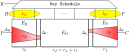
\includegraphics[width=\textwidth]{./figures/KB3.pdf}}
\end{figure}
\end{frame}

\begin{frame}
\begin{center}
\vspace{2.5cm}
{\huge \faLaptop~Demo~2}
\end{center}
\end{frame}

\section{Conclusion}
\sectionheader[\huge\color{tug}\faClockO]{Conclusion}

\begin{frame}{Our Main Contributions}
\begin{itemize}
\item[\faCheckCircleO] We introduced a unified CP model for full ID/ZC/Integral attacks
\item[\faCheckCircleO] We applied our method to \cipher{SKINNY}, \cipher{CRAFT}, \cipher{SKINNYe}, and \cipher{SKINNYee} and improved their ID/ZC/Integral attacks significantly
\item[\faCheckCircleO] Our method is generic and can be applied to other strongly aligned block ciphers, e.g., \cipher{AES}
\end{itemize}

\begin{center}
\vspace{0.44cm}

{\large Thanks for your attention!}

\faGithub: \url{https://github.com/hadipourh/talks}\\
\vspace{0.35cm}
\faArchive: \url{https://ia.cr/2022/1147}
\end{center}
\end{frame}

%%%%%%%%%%%%%%%%%%%%%%%%%%%%%%%%%%%%%%%%%%%%%%%%%%%%%%%%%%%%%%%%%%%%%%%%%%%%

\begin{frame}[allowframebreaks]{Bibliography}
  \printbibliography
\end{frame}

\begin{filecontents*}[overwrite]{\jobname.bib}

% seminal paper of ZC attack
@article{dcc_BogdanovR14,
  author    = {Andrey Bogdanov and
               Vincent Rijmen},
  title     = {Linear hulls with correlation zero and linear cryptanalysis of block
               ciphers},
  journal   = {Des. Codes Cryptogr.},
  volume    = {70},
  number    = {3},
  pages     = {369--383},
  year      = {2014},
  doi       = {10.1007/s10623-012-9697-z}
}

% seminal paper of multipl ZC attacks
@inproceedings{fse_BogdanovW12,
  author    = {Andrey Bogdanov and
               Meiqin Wang},
  title     = {Zero Correlation Linear Cryptanalysis with Reduced Data Complexity},
  booktitle = {{FSE} 2012},
  series    = {Lecture Notes in Computer Science},
  volume    = {7549},
  pages     = {29--48},
  publisher = {Springer},
  year      = {2012},
  doi       = {10.1007/978-3-642-34047-5_3}
}

% multidimensional zc and link between zc and integral attacks
@inproceedings{asiacrypt_BogdanovLNW12,
  author    = {Andrey Bogdanov and
               Gregor Leander and
               Kaisa Nyberg and
               Meiqin Wang},
  title     = {Integral and Multidimensional Linear Distinguishers with Correlation
               Zero},
  booktitle = {{ASIACRYPT} 2012},
  series    = {Lecture Notes in Computer Science},
  volume    = {7658},
  pages     = {244--261},
  publisher = {Springer},
  year      = {2012},
  doi       = {10.1007/978-3-642-34961-4_16}
}

% integral attack as a theoretical generalization of differential cryptanalysis
@article{Lai1994,
  author      =  {Lai, Xuejia},
  editor      = {Blahut, Richard E.
                and Costello, Daniel J.
                and Maurer, Ueli
                and Mittelholzer, Thomas},
  title       = {Higher Order Derivatives and Differential Cryptanalysis},
  booktitle   = {Communications and Cryptography: Two Sides of One Tapestry},
  year        = {1994},
  publisher   = {Springer US},
  address     = {Boston, MA},
  pages       = {227--233},
  doi         = {10.1007/978-1-4615-2694-0_23},
}

% integral attack by Daemen
@inproceedings{square_fse_DaemenKR97,
  author    = {Joan Daemen and
               Lars R. Knudsen and
               Vincent Rijmen},
  title     = {The Block Cipher {Square}},
  booktitle = {{FSE} 1997},
  series    = {LNCS},
  volume    = {1267},
  pages     = {149--165},
  publisher = {Springer},
  year      = {1997},
  doi       = {10.1007/BFb0052343},
}

% link between ZC, ID and Integral attacks
@inproceedings{crypto_SunLRLCWAL15,
  author    = {Bing Sun and
               Zhiqiang Liu and
               Vincent Rijmen and
               Ruilin Li and
               Lei Cheng and
               Qingju Wang and
               Hoda AlKhzaimi and
               Chao Li},
  title     = {Links Among Impossible Differential, Integral and Zero Correlation
               Linear Cryptanalysis},
  booktitle = {{CRYPTO} 2015},
  series    = {Lecture Notes in Computer Science},
  volume    = {9215},
  pages     = {95--115},
  publisher = {Springer},
  year      = {2015},
  doi       = {10.1007/978-3-662-47989-6_5}
}

% milp-based method to search for ID attacks - works for SPN
@inproceedings{eurocrypt_SasakiTodo2017,
  author    = {Sasaki, Yu
              and Todo, Yosuke},              
  editor    = {Coron, Jean-S{\'e}bastien
              and 
              Nielsen, Jesper Buus},
  title     = {New Impossible Differential Search Tool from Design and Cryptanalysis Aspects},
  Xbooktitle = {Advances in Cryptology -- EUROCRYPT 2017},
  booktitle = {{EUROCRYPT} 2017},
  year      = {2017},
  publisher = {Springer International Publishing},
  address   = {Cham},
  pages     = {185--215},
  doi       = {10.1007/978-3-319-56617-7_7}
}

% milp-based method to search for ID attacks - works for ARX and SPN
@misc{eprint_Cui,
  author    = {Tingting Cui and 
            Shiyao Chen and 
            Keting Jia and 
            Kai Fu and 
            Meiqin Wang},
  title     = {New Automatic Search Tool for Impossible Differentials and Zero-Correlation Linear Approximations},
  howpublished = {Cryptology ePrint Archive, Paper 2016/689},
  year      = {2016},
  note      = {\url{https://eprint.iacr.org/2016/689}},
  url       = {https://eprint.iacr.org/2016/689}
}

% cp-based method by sun and gerault
@article{tosc_SunGLYTQH2017,
author      = {Sun, Siwei and 
            Gerault, David and 
            Lafourcade, Pascal and 
            Yang, Qianqian and 
            Todo, Yosuke and 
            Qiao, Kexin and 
            Hu, Lei}, 
  title     = {Analysis of AES, SKINNY, and Others with Constraint Programming}, 
  volume    = {2017}, 
  doi       = {10.13154/tosc.v2017.i1.281-306}, 
  number    = {1}, 
  journal   = {IACR Transactions on Symmetric Cryptology}, 
  year      = {2017}, 
  month     = {Mar.}, 
  pages     = {281–306} 
}

% cp model to encode the deterministic truncated trails
@article{tosc_SunGWW2020, 
  author    = {Sun, Ling and Gerault, David and Wang, Wei and Wang, Meiqin},
  title     = {On the Usage of Deterministic (Related-Key) Truncated Differentials and Multidimensional Linear Approximations for SPN Ciphers}, 
  volume    = {2020},   
  doi       = {10.13154/tosc.v2020.i3.262-287}, 
  number    = {3}, 
  journal   = {IACR Transactions on Symmetric Cryptology}, 
  year      = {2020}, 
  month     = {Sep.}, 
  pages     = {262–287}
}

% patrick's tool for mitm and id attacks
@inproceedings{crypto_DerbezF16,
  author    = {Patrick Derbez and
               Pierre{-}Alain Fouque},
  title     = {Automatic Search of Meet-in-the-Middle and Impossible Differential
               Attacks},
  booktitle = {{CRYPTO} 2016},
  series    = {Lecture Notes in Computer Science},
  volume    = {9815},
  pages     = {157--184},
  publisher = {Springer},
  year      = {2016}
}

% skinny specification
@inproceedings{skinny,  
  author    = {Beierle, Christof and 
              Jean, J{\'e}r{\'e}my and 
              K{\"o}lbl, Stefan and 
              Leander, Gregor and 
              Moradi, Amir and 
              Peyrin, Thomas and 
              Sasaki, Yu and 
              Sasdrich, Pascal and 
              Sim, Siang Meng},
  title     = {{The SKINNY family of block ciphers and its low-latency variant MANTIS}},
  Xbooktitle= {Advances in Cryptology -- CRYPTO 2016},
  booktitle = {{CRYPTO} 2016},
  pages     = {123--153},
  year      = {2016},
  organization= {Springer},
  doi       = {10.1007/978-3-662-53008-5_5},
}

% specification of ZUC
@article{zuc128_specification,
	author    = {ETSI/SAGE},
	title     = {Specification of the 3GPP confidentiality and integrity algorithms
	{128-EEA3} and {128-EIA3}: {ZUC} specification},
	journal   = {ETSI/SAGE, Document 2, Version 1.6},
	year      = {2011}
}

@article{zuc256_specification,
	author    = {ZUC Design Team},
	title     = {The {ZUC}-256 Stream Cipher},
	year      = {2018},
	note      = {\url{http://www.is.cas.cn/ztzl2016/zouchongzhi/201801/W020180126529970733243.pdf}}
}

@article{ascon_caesar_submission_2016,
	title     = {Ascon v1.2},
	author    = {Dobraunig, Christoph and Eichlseder, Maria and Mendel, Florian and Schl{\"a}ffer, Martin},
	journal   = {Submission to the CAESAR Competition},
	year      = {2016}
}

% specification of AES
@article{daemen1999aes,
	title     = {{AES} proposal: {Rijndael}},
	author    = {Daemen, Joan and Rijmen, Vincent},
	year      = {1999},
	note      = {\url{https://csrc.nist.gov/csrc/media/projects/cryptographic-standards-and-guidelines/documents/aes-development/rijndael-ammended.pdf}}
}

% specification of CLEFIA
@inproceedings{conf_fse_ShiraiSAMI07,
  author    = {Taizo Shirai and
               Kyoji Shibutani and
               Toru Akishita and
               Shiho Moriai and
               Tetsu Iwata},
  title     = {The 128-Bit Blockcipher {CLEFIA} (Extended Abstract)},
  booktitle = {{FSE} 2007},
  series    = {LNCS},
  volume    = {4593},
  pages     = {181--195},
  publisher = {Springer},
  year      = {2007}
}

% specification of TRIVIUM
@incollection{canniere2008trivium,
  title     = {Trivium},
  author    = {Canni{\`e}re, Christophe De and Preneel, Bart},
  booktitle = {New stream cipher designs},
  pages     = {244--266},
  year      = {2008},
  publisher = {Springer}
}

% specification of Enocoro-128v2
@article{watanabe2010hardware,
  title     = {A Hardware-Oriented Light Weight Pseudo-Random Number Generator Enocoro-128v2. The 2010 Symposium on Cryptography and Information Security, SCIS 2010, 3D1-3},
  author    = {Watanabe, D and Okamoto, K and Kaneko, T},
  year      = {2010}
}

% specification of Keccak
@inproceedings{eurocrypt_BertoniDPA13,
  author    = {Guido Bertoni and
               Joan Daemen and
               Micha{\"{e}}l Peeters and
               Gilles Van Assche},
  title     = {Keccak},
  booktitle = {{EUROCRYPT}},
  series    = {Lecture Notes in Computer Science},
  volume    = {7881},
  pages     = {313--314},
  publisher = {Springer},
  year      = {2013},
  doi       = {10.1007/978-3-642-38348-9_19}
}

% full break of MISTY1
@inproceedings{conf_crypto_Todo15,
	author    = {Yosuke Todo},
	title     = {Integral Cryptanalysis on Full {MISTY1}},
	booktitle = {{CRYPTO} 2015},
	series    = {Lecture Notes in Computer Science},
	volume    = {9215},
	pages     = {413--432},
	publisher = {Springer},
	year      = {2015},
  doi       = {10.1007/s00145-016-9240-x}
}

% full break of DES
@inproceedings{conf_eurocrypt_Matsui93,
	author    = {Mitsuru Matsui},
	title     = {Linear Cryptanalysis Method for {DES} Cipher},
	booktitle = {{EUROCRYPT} 1993},
	series    = {Lecture Notes in Computer Science},
	volume    = {765},
	pages     = {386--397},
	publisher = {Springer},
	year      = {1993},
  doi       = {10.1007/3-540-48285-7_33}
}

% cube attack on Keccak
@inproceedings{conf_eurocrypt_HuangWXWZ17,
	author    = {Senyang Huang and
	Xiaoyun Wang and
	Guangwu Xu and
	Meiqin Wang and
	Jingyuan Zhao},
	title     = {Conditional Cube Attack on Reduced-Round Keccak Sponge Function},
	booktitle = {{EUROCRYPT} 2017},
	series    = {Lecture Notes in Computer Science},
	volume    = {10211},
	pages     = {259--288},
	year      = {2017},
  doi       = {10.1007/978-3-319-56614-6_9}
}

% related-key boomerang attack on AES
@inproceedings{conf_crypto_BiryukovKN09,
	author    = {Alex Biryukov and
	Dmitry Khovratovich and
	Ivica Nikolic},
	title     = {Distinguisher and Related-Key Attack on the Full {AES-256}},
	booktitle = {{CRYPTO} 2009},
	series    = {Lecture Notes in Computer Science},
	volume    = {5677},
	pages     = {231--249},
	publisher = {Springer},
	year      = {2009}
}

@inproceedings{asiacrypt_XiangZBL16,
  author    = {Zejun Xiang and
               Wentao Zhang and
               Zhenzhen Bao and
               Dongdai Lin},
  title     = {Applying {MILP} Method to Searching Integral Distinguishers Based
               on Division Property for 6 Lightweight Block Ciphers},
  booktitle = {{ASIACRYPT} 2016},
  series    = {Lecture Notes in Computer Science},
  volume    = {10031},
  pages     = {648--678},
  year      = {2016},
  doi       = {10.1007/978-3-662-53887-6_24}
}

@article{tosc_BeierleLMR19,
  author    = {Christof Beierle and
               Gregor Leander and
               Amir Moradi and
               Shahram Rasoolzadeh},
  title     = {{CRAFT:} Lightweight Tweakable Block Cipher with Efficient Protection
               Against {DFA} Attacks},
  journal   = {{IACR} Trans. Symmetric Cryptol.},
  volume    = {2019},
  number    = {1},
  pages     = {5--45},
  year      = {2019},
  doi       = {10.13154/tosc.v2019.i1.5-45}
}

\end{filecontents*}

\end{document}
